\chapter{2023年\textsf{HDU}「普通物理1」期中试题解答}

\begin{minipage}{0.32\textwidth}
    \textbf{开课学院}：理学院
      
    \textbf{课程编码}：A0715011s
\end{minipage}
\hfill
\begin{minipage}{0.32\textwidth}
    \textbf{解析制作}：\textsc{Mingyu Hsia}

    \textbf{\,\hologo{TeX}~排版}：\textsc{Mingyu Hsia}
\end{minipage}
\hfill
\begin{minipage}{0.15\textwidth}
    \centering
    \begin{tikzpicture}
        \node [inner sep=0] at (0,0) {
            \qrcode[height=3em,version=4]{https://qm.qq.com/q/Jd5GTWrMAs}};
        \fill [color=white,rounded corners=(sqrt(2)+2)/11*1em] (-.5em,-.5em) rectangle (.5em,.5em);
        \node [inner sep=0] at (0,0) {\color{MidnightBlue}\scriptsize\faIcon{qq}};
    \end{tikzpicture}

    \scriptsize\href{https://qm.qq.com/q/Jd5GTWrMAs}{\itshape 未央物理营\! $^\dagger$}
\end{minipage}
\hfill
\begin{minipage}{0.15\textwidth}
    \centering
    \begin{tikzpicture}
        \node [inner sep=0] at (0,0) {
            \qrcode[height=3em,version=4]{http://weixin.qq.com/r/DBIABcHEqgnWKIVmb0eI}};
            \fill [color=white,rounded corners=(sqrt(2)+2)/11*1em] (-.5em,-.5em) rectangle (.5em,.5em);
        \node [inner sep=0] at (0,0) {\color{DarkGreen}\scriptsize\faIcon{weixin}};
    \end{tikzpicture}

    \scriptsize\href{http://weixin.qq.com/r/DBIABcHEqgnWKIVmb0eI}{\itshape 未央学社}
\end{minipage}

\section{选择题（每题3分，共30分）}

\begin{problem}
    根据瞬时速度矢量$\bm v$的定义，在直角坐标系下，其大小$\abs{\bm v}$可表示为
    \begin{tasks}(2)
        \task $\displaystyle\odv rt$
        \task $\displaystyle\abs{\odv xt\bm i}+\abs{\odv yt\bm j}+\abs{\odv zt\bm k}$
        \task[\true] $\displaystyle\sqrt{\ab(\odv xt)^2+\ab(\odv yt)^2+\ab(\odv zt)^2}$
        \task $\displaystyle\odv xt+\odv yt+\odv zt$
    \end{tasks}
\end{problem}
\solute3
\begin{solution}
    直角坐标下速度的大小即其三个方向分量的平方和的算数平方根.
\end{solution}

\begin{paracol}{2}
\begin{problem}{转动惯量}
    如图所示，质量为$m$的均质杆长为$l$，绕铅直轴$OO'$成$\theta$角转动，转动惯量为
    \begin{tasks}(10)
        \task*(2) $ml^2/12$
        \task*(3) $ml^2\sin^2\theta/4$
        \task*(3)[\true] $ml^2\sin^2{\theta}/3$
        \task*(2) $ml^2/3$
    \end{tasks}
\end{problem}
\switchcolumn
\centering
\begin{tikzpicture}[scale=.9]
    \draw [thick] ellipse (1.5 and .5);
    \draw [thick] (0,-2.2) node [left] {$O$} -- (0,-0.5) (0,0) coordinate (c) -- (0,1)  node [left] {$O'$};
    \draw [very thick] (0,-2) coordinate (b) -- (1.5,0) coordinate (a) node[below right,midway] {$l$};
    \pic["$\theta$", draw=red!80!green!60!, ultra thick, angle eccentricity=1.5, angle radius=18]{angle=a--b--c};
\end{tikzpicture}
\switchcolumn
\begin{solution}
    $I=\int_0^lr^2\d m=\int_0^l(x\sin\theta)^2\lambda\d x=ml^2\sin^2\theta/3$.
\end{solution}
\end{paracol}

\begin{problem}
    将细绳绕在一个具有水平光滑轴的飞轮边缘上，现在绳端挂一质量为$m$的重物，飞轮的角加速度为$\alpha$. 如果以拉力$2mg$代替重物拉绳时，飞轮的角加速度将
    \begin{tasks}(4)
        \task 小于$2\alpha$
        \task 大于$\alpha$，小于$2\alpha$
        \task[\true] 大于$2\alpha$
        \task 等于$2\alpha$
    \end{tasks}
\end{problem}
\solute1
\begin{note}\leavevmode
\begin{itemize}
    \item 下落过程中物体也要增加自己的动能，所以会``拖累''滑轮的加速转动过程. 所以直接用拉力$P$去拉绳子使滑轮获得的角加速度要比重物带着绳子使滑轮获得的角加速度大.
    \item 重物加速下落的过程中属于失重过程，绳子的拉力一定小于其重力$P$，进而拉力对滑轮的力矩就小于$PR$，所以前者角加速度要比后者小，即直接用拉力$P$去拉绳子使滑轮获得的角加速度要比重物带着绳子使滑轮获得的角加速度大.
\end{itemize}
\end{note}
\begin{solution}
设绳子拉力为$T$. 对重物列牛顿运动定律、对滑轮列转动定律得
\[\begin{cases}
    mg-T=ma\\
    TR=I\alpha
\end{cases}\]
由线量和角量之间的关系$a=R\alpha$联立以上两式得$2\alpha=2mgR/(mR^2+I)<2mgR/I$.
\end{solution}

\begin{problem}
\begin{paracol}{2}
    如图所示，一个小物体，位于光滑的水平桌面上，与一绳的一端相连结，绳的另一端穿过桌面中心的小孔$O$. 该物体原以角速度$\omega$在半径为$R$的圆周上绕$O$旋转，今将绳从小孔缓慢往下拉. 则物体
    \switchcolumn\vspace*{\fill}\centering
    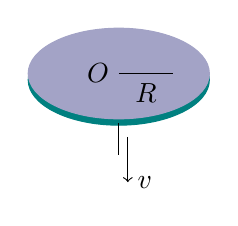
\begin{tikzpicture}[scale=1.15]
        \filldraw [yshift=-2,teal] (0,0) ellipse (1 and .5);
        \filldraw [MidnightBlue!40!] (0,0) ellipse (1 and .5);
        \draw (0,0) -- (.6,0);
        \draw (0,-.55) -- (0,-.9);
        \node [left] at (0,0) {$O$};
        \node [below] at (.3,0) {$R$};
        \draw [->] (.1,-.7) -- (.1,-1.2);
        \node [right] at (.1,-1.2) {$\bm v$};
    \end{tikzpicture}\vspace*{\fill}
\end{paracol}
\begin{tasks}(2)
    \task 动能不变，动量改变
    \task 动量不变，动能改变
    \task 角动量不变，动能不变
    \task[\true] 角动量不变，动能、动量都改变
\end{tasks}
\end{problem}
\solute2
\begin{solution}
    物体所受合力不等于零，动量改变. 受力始终指向$O$，其力矩为零，角动量不变. 下拉过程中物体运动半径减小，速度增大，动能变大.
\end{solution}

\begin{problem} % [速度、加速度]
    一个质点作直线运动，某时刻的瞬时速度$v=\qty2{\m/\s}$，瞬时加速度$a=\qty{-2}{\m/\s^2}$，则一秒钟后质点的速度
    \begin{tasks}(4)
        \task 等于零
        \task 等于$\qty{-2}{\m/\s}$
        \task 等于$\qty2{\m/\s}$
        \task[\true] 不能确定
    \end{tasks}
\end{problem}
\vspace{-.75em}
\begin{solution}
    由于题目中未强调质点的加速度是否为常数，所以一秒钟后质点的速度不能确定.
\end{solution}

\begin{paracol}{2}
\begin{problem}
    均匀细棒$OA$可绕通过其一端$O$而与棒垂直的水平固定光滑轴转动，如图所示. 今使棒从水平位置由静止开始自由下落，在棒摆动到竖直位置的过程中，角动量$L$与角加速度$\beta$的变化趋势分别为
    \begin{tasks}(2)
    \task $L$减小，$\beta$减小
    \task $L$减小，$\beta$增大
    \task $L$增大，$\beta$增大
    \task[\true] $L$增大，$\beta$减小
    \end{tasks}
    \switchcolumn\vspace*{\fill}\centering
    \begin{tikzpicture}[scale=.8]
        \wall{(-.8,.25)}{(.8,.4)};
        \draw (-.1,-4.2) rectangle + (.2,4);
        \draw [dashed] (-.1,-.4) rectangle +(4,.2);
        \draw [rounded corners=3pt] (-.3,.25) -- (0,-.4) -- (.3,.25);
        \filldraw (0,-.3) circle (.05);
        \node [below left] at (0,-.3) {$O$};
        \node [right] at (3.9,0) {$A$};
    \end{tikzpicture}\vspace*{\fill}
\end{problem}
\end{paracol}
\solute2
\begin{solution}
    下落过程中，细棒的角速度不断增大，所以其角动量由小到大；刚释放时，其所受重力矩为$mgl/2$，摆动到竖直位置时，其所受重力矩为零，所以其角加速度由大到小.
\end{solution}

\begin{problem}
    两个同心薄金属球壳，半径分别为$R_1$和$R_2$，且$R_2>R_1$. 若分别带上电量为$q_1$和$q_2$，则两者的电势分别为$\varphi_1$和$\varphi_2$（选无穷远处为电势零点）. 现用导线将两球壳相连接，则它们的电势
    \begin{tasks}(4)
        \task $\varphi_1$
        \task $\varphi_2$
        \task $\varphi_1+\varphi_2$
        \task $(\varphi_1+\varphi_2)/2$
    \end{tasks}
\end{problem}
\begin{solution}
    $\varphi_2=q_1/4\pi\epsilon_0R_2+q_2/4\pi\epsilon_0R_2=(q_1+q_2)/4\pi\epsilon_0R_2$. 连接后电荷全部转移到外球壳表面，所以它们的电势为$\varphi_2$.
\end{solution}

\begin{problem}
    真空中两块互相平行的无限大均匀带电平面，其电荷密度分别为$+\sigma$和$+2\sigma$，两板之间的距离为$d$，两板间的电场强度大小
    \begin{tasks}(4)
        \task $0$
        \task $3\sigma/2\epsilon_0$
        \task $\sigma/\epsilon_0$
        \task $\sigma/2\epsilon_0$
    \end{tasks}
\end{problem}
\begin{solution}
    由无限大均匀带电平面附近场强公式得板间场强大小$E=2\sigma/2\epsilon_0-\sigma/2\epsilon_0=\sigma/2\epsilon_0$.
\end{solution}

\begin{paracol}{2}
\begin{problem}
    如图所示，$CDEF$是一矩形，边长分别为$l$和$2l$. 在$DC$延长线上$CA=l$处的$A$点有点电荷$+q$，在$CF$的中点$B$点有点电荷$-q$. 若使单位正电荷从$C$点沿$CDEF$路径运动到$F$点，则电场力所做的功等于
    \begin{tasks}(2)
        \task $(\sqrt5-1)q/4\pi\epsilon_0l(\sqrt5-l)$
        \task $(1-\sqrt5)q/4\pi\epsilon_0l\sqrt5-l$
        \task $(\sqrt3-1)q/4\pi\epsilon_0l(\sqrt3)$
        \task $(\sqrt5-1)q/4\pi\epsilon_0l(\sqrt5)$
    \end{tasks}
    \switchcolumn\centering
    \begin{tikzpicture}[scale=1.5]
        \draw (0,-1) -- (0,1) node [left,midway] {$C$} node [above left] {$D$} -- (2,1) node [above right] {$E$} -- (2,0) node [right] {$F$} -- (0,0);
        \shade [ball color=MidnightBlue!50] (0,-1) circle (.05) node [right] {$A$} node [below] {$+q$};
        \shade [ball color=MidnightBlue!50] (1,0) circle (.05) node [below] {$B$} node [above] {$-q$};
        \length{(-.5,-1)}{(-.5,0)}{$L$}{(0,.5)};
        \length{(-.5,0)}{(-.5,1)}{$L$}{(0,.5)};
        \length{(0,-.5)}{(1,-.5)}{$L$}{(.5,0)};
        \length{(1,-.5)}{(2,-.5)}{$L$}{(.5,0)};
    \end{tikzpicture}
\end{problem}
\end{paracol}
\begin{solution}
    由于电场力是保守力，单位正电荷移动前后与$-q$的距离相等，$-q$产生的电场对其不做功. 以$A$为原点，水平向右为$x$轴方向. 电场力做功等于单位正电荷在$+q$产生的电场中电势能的负变化量
    \[W=-(\varphi_F-\varphi_A)=\frac{q}{4\pi\epsilon_0l}-\frac{q}{4\pi\epsilon_0\sqrt5l}=\frac{(\sqrt5-1)q}{4\pi\epsilon_0\sqrt5l}\]
\end{solution}

\begin{problem}
    真空中有``孤立的''均匀带电球体和一个均匀带电球面，如果它们的半径和所带的电荷都相等，则它们的能之间的关系是
    \begin{tasks}(3)
        \task 球体静电能等于球面静电能
        \task[\true] 球体静电能大于球面静电能
        \task 球体静电能小于球面静电能
        \task! 球体内静电能大于球面静电能，球体外静电能大于球面静电能
    \end{tasks}
\end{problem}
\begin{solution}
    根据高斯定理，两球外电场分布相同，电场能量相等. 但球面内电场为零，球体内电场不为零，所以球体内部有电场能，球面内部没有电场能. 所以球体静电能大于球面静电能.
\end{solution}

\section{填空题（共20分）}

\begin{problem}
    质量为$m$的物体，初速极小，在外力作用下从原点起沿$x$轴正向运动. 所受外力方向沿$x$轴正向，大小为$F=kx$. 物体从原点运动到点$x_0$的过程中所受外力冲量的大小为\ans{$\sqrt{mkx^2}$}.
\end{problem}
\begin{solution}
    由动能定理$mv^2/2=\int_0^{x_0}kx\d x$得$v=\sqrt{kx^2/m}$，所以物体所受外力冲量的大小为$I=mv=\sqrt{mkx^2}$.
\end{solution}

\begin{problem}
    转动着的飞轮的转动惯量为$I$，在$t=0$时角速度为$\omega_0$. 此后飞轮经历制动过程，阻力矩$M$的大小与角速度$\omega$的平方成正比，比例系数为$k$（$k>0$）. 当$\omega=\omega_0/3$时，飞轮的角加速度\ans{$-k\omega_0^2/9I$}.
\end{problem}
\solute0
\begin{solution}
    由转动定律$-k\omega^2=I\beta$，当$\omega=\omega_0/3$时，角加速度为$\beta=-k\omega_0^2/9I$.
\end{solution}

\begin{problem}
    长为$l$、质量为$M$的匀质杆可绕通过杆一端$O$的水平光滑固定轴转动，开始时杆竖直下垂. 一质量为$m$的子弹以水平速度$\bm v_0$射入杆上$A$点，并嵌在杆中，$\overline{OA}=2l/3$，则子弹射入后瞬间杆的角速度$\omega=$\ans{$6v_0/7l$}.
\end{problem}
\begin{solution}
    由子弹和杆组成的系统对$O$点角动量守恒$mv_0\cdot2l/3=[ml^2/3+m(2l/3)^2]\omega$得入射后杆的角速度$\omega=6v_0/7l$.
\end{solution}

\begin{problem}
    质量为$m$的小球，用轻绳$AB$、$BC$连接，如左下图所示，其中$AB$水平，剪断绳$AB$前后的瞬间，绳$BC$中的张力比$T:T'=$\ans{$1:\cos^2\theta$}.
\end{problem}
\solute1
\begin{solution}    
    剪断前后，$m$分别沿竖直方向和绳方向受力平衡，即$T\cos\theta=mg$，$mg\cos\theta=T'$. 解得$T:T'=1:\cos^2\theta$.
\end{solution}

\begin{figure}[htbp]
    \begin{minipage}{.3\textwidth}
        \centering
        \begin{tikzpicture}[scale=.6]
            \draw [ultra thick] (-2,2.5) -- (1.2,2.5);
            \draw [ultra thick] (-2,2.5) -- (-2,-.5);
            \draw (1,2.5) coordinate (c) node [above] {$C$} -- (0,0) coordinate (b) node [right] {$B$} node [above left] {$m$} -- (-2,0) node [left] {$A$};
            \draw [dashed] (1,2.5) -- (1,-.5) coordinate (d);
            \shade[ball color = MidnightBlue] (0,0) circle (.1);
            \draw [MidnightBlue,very thick,->] (0,0) -- (-.8,0);
            \draw [MidnightBlue,very thick,->] (0,0) -- (.8,2) node [left] {$T$};
            \draw [MidnightBlue,very thick,->] (0,0) -- (0,-2) node [right] {$mg$};
            \draw [MidnightBlue,very thick,->] (0,0) -- (.512,1.28) node [left] {$T'$};
            \pic["$\theta$",draw=DarkRed,ultra thick,angle eccentricity=1.5,angle radius=18]{angle=b--c--d};
        \end{tikzpicture}
    \end{minipage}
    \hfill
    \begin{minipage}{.3\textwidth}
        \centering
        \begin{tikzpicture}[scale=.6]
            \draw (0,0) circle (2);
            \draw [->] (-2,0) node [left] {$P$} -- (0,0) node [above] {$O$} -- (1,{sqrt(3)}) node [above right] {$R$};
            \filldraw (-2,0) circle (.05);
            \filldraw [pattern=north east lines] (-.8,-.1) -- (-.8,.1) -- (.8,.1) -- (.8,-.1)--cycle;
            \length{(-.8,-.5)}{(.8,-.5)}{$L$}{(.5,0)};
        \end{tikzpicture}
    \end{minipage}
    \hfill
    \begin{minipage}{.3\textwidth}
        \centering
        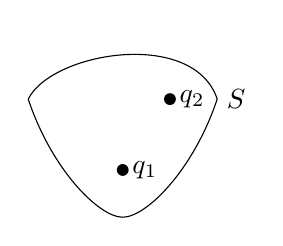
\begin{tikzpicture}[scale=1.5]
            \draw(-.8,.4) .. controls (-.6,.8) and (.6,1) .. (.8,.4) node [right] {$S$} .. controls (.6,-.2) and (.2,-.6) .. (0,-.6) .. controls (-.2,-.6) and (-.6,-.2) .. (-.8,.4);
            \fill (0,-.2) circle (.05) node [right] {$q_1$};
            \fill (.4,.4) circle (.05) node [right] {$q_2$};
        \end{tikzpicture}
    \end{minipage}
\end{figure}

\begin{problem} % {高斯定理}
    一均匀带电直导线长为$L$，电荷线密度为$+\gamma$.过导线中点$O$作一半径为$R$（$R>L/2$）的球面$S$，$P$为带电直导线的延长线与球面$S$的交点.则通过该球面的电场强度通量$\Phi_e=$\ans{$\gamma L/\epsilon_0$}.
\end{problem}
\begin{solution}
    由高斯定理得$\Phi_e=\gamma L/\epsilon_0$.
\end{solution}

\begin{problem}
    带电量分别为$q_1$和$q_2$的两个点电術单独在空间各点产生的静电场强分别为$\bm E_1$和$\bm E_2$，空间各点的总的电场强度为$\bm E=\bm E_1+\bm E_2$，现在作一封闭曲面$S$，如右上图所示，则以下两式可分别求出通过$S$的电通量$\oiint_S\bm E_1\cdot\d\bm S=$\ans{$q_1/\epsilon_0$}，$\oiint_S\bm E\cdot\d\bm S=$\ans{$(q_1+q_2)/\epsilon_0$}.
\end{problem}
\solute0

\section{计算题（共50分）}

\begin{paracol}{2}
\begin{problem}
    如图所示，两个大小不同、具有水平光滑轴的定滑轮，定点在同一水平线上. 小滑轮的质量为$m$，半径$r$，对轴的转动惯量$I=mr^2/2$，大滑轮的质量$m'=2m$、半径$r'=2r$，对轴的转动惯量$I'=m'r'^2/2$. 一根不可伸缩的轻质细绳跨过两个定滑轮，绳的两端分别挂着物体$A$和$B$. $A$的质量为$m$，$B$的质量为$m'=2m$. 这一系统由静止开始转动. 求两滑轮的角加速度和它们之间绳子的张力.
    \switchcolumn\vspace*{\fill}\centering
    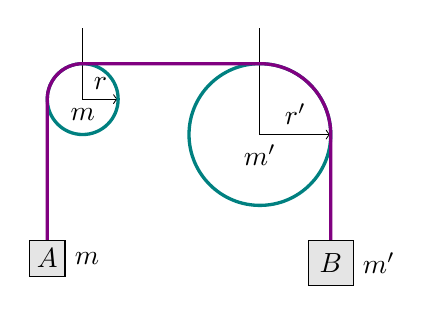
\begin{tikzpicture}[scale=.9]
        \wall{(-1.2,1)}{(4.2,1.2)};
        \draw [->] (0,1) -- (0,0) node [below] {$m$} -- (.5,0) node [midway,above] {$r$};
        \draw [very thick,teal] (0,0) circle (.5);
        \draw [->] (2.5,1) -- (2.5,-.5) node [below] {$m'$} -- (3.5,-.5) node [midway,above] {$r'$};
        \draw [very thick,teal] (2.5,-.5) circle (1);
        \draw [very thick,color=violet] (-.5,-2) -- (-.5,0) arc (180:90:.5) -- (2.5,.5) arc (90:0:1) -- (3.5,-2);
        \filldraw [gray!20,draw=black] (-.75,-2) rectangle (-.25,-2.5) node [black,midway] {$A$} node [black,right] at (-.25,-2.25) {$m$};
        \filldraw [gray!20,draw=black] ({3.5-.5*2^(1/3)/2},-2) rectangle + ({.5*2^(1/3)},{-.5*2^(1/3)}) node [black,midway] {$B$} node [black,right] at ({3.5+.5*2^(1/3)/2},{-2-.5*2^(1/3)/2}) {$m'$};
    \end{tikzpicture}\vspace*{\fill}
\end{problem}
\end{paracol}
\solute{-2}
\begin{multicols}{2}
\begin{solution}
    设二者之间绳子的张力为$T$，悬挂$A$、$B$绳子的张力分别为$T_A$、$T_B$. 对$A$，$B$和两个滑轮，分别由牛顿运动定律和转动定律得
    \[\begin{cases}
        T_A-mg=ma\\
        m'g-T_B=m'a\\
        Tr-T_Ar=I\beta_1\\
        T_Br'-Tr'=I'\beta_2
    \end{cases}\]
    利用关系$\beta_1r=\beta_2r'=a$联立以上五式得
    \begin{itemize}
        \item $\displaystyle\beta_1=\frac{(m'-m)g}{(m+m')r+I/r+I'r/r'^2}$
        \item $\displaystyle\beta_2=\frac{(m'-m)g}{(m+m')r'+Ir'/r^2+I'/r'}$
        \item $\displaystyle a=\frac{(m'-m)g}{m+m'+I/r^2+I'/r'^2}$
        \item $T=ma+mg+Ia/r^2$
    \end{itemize}
\end{solution}
\end{multicols}

\begin{problem}
    光滑平面上并排静放着两块质量分别为$m_1$和$m_2$的木块，一质量为$m_0$的子弹以$v_0$的初速度水平射向两木块，若$m_1=2m_0$，$m_2=m_0$，子弹水平射穿$m_1$后，射入$m_2$内. 当子弹相对$m_2$静止时，$m_2$的速度是$m_1$的二倍. 求此过程中摩擦阻力所做的功.
\end{problem}
\begin{solution}
    子弹、$m_1$和$m_2$组成的系统在水平方向上动量守恒. 设当子弹相对$m_2$静止时$m_1$的速度大小为$v$
    \[m_0v_0=m_1v+(m_2+m_0)\cdot2v\]
    得此时$m_1$的速度大小$v=m_0v_0/[m_1+2(m_2+m_0)]=v_0/6$. 由能量守恒定律得摩擦阻力所做的功$W_f=m_0v_0^2/2-m_1v^2/2-(m_2+m_0)\cdot(2v)^2/2=13mv_0^2/36$.
\end{solution}

\begin{problem}
    一根放在水平光滑桌面上的匀质棒，可绕通过其一端的竖直固定光滑轴$O$转动. 棒的质量为$m=\qty{1.5}\kg$，长为$l=\qty{1.0}\m$，对轴的转动惯量为$I=ml^2/3$，初始时棒静止. 有一水平运动的子弹垂直射入棒的$A$端，并留在棒中. 子弹的质量为$m'=\qty{0.02}\kg$，速率为$v=\qty{400}{\m/\s}$. 试问
    \begin{enumerate}
        \item 棒开始和子弹一起转动时角速度$\omega$有多大？
        \item 若棒转动时受到大小为$M_r=\qty{4.0}{\N\cdot\m}$的恒定阻力矩作用，棒能转过多大的角度$\theta$？
    \end{enumerate}
\end{problem}
\begin{solution}\leavevmode
    \begin{enumerate}
        \item 由子弹和棒组成的系统对$O$点角动量守恒$m'v_0l=(ml^2/3+m'l^2)\omega$得入射后棒的角速度$\omega=3m'v_0/(3m'+m)l=\qty{15.38}{\radian/\s}$.
        \item 由动能定理$M_r\theta=\frac12(ml^2/3+m'l^2)\omega^2$得棒能转过的角度$\theta=\qty{15.38}{\radian}$.
    \end{enumerate}
\end{solution}

\begin{problem}
    真空中一个半径为$R$的带电球，其电荷体密度$\rho=kr^2$，其中$k$是正常数，$r$是离球心的距离. 求带电球体在空间的电场分布.
\end{problem}
\begin{solution}
    由高斯定理得带电球体在空间的电场分布为
    \[\begin{cases}
        E\cdot4\pi r^2=\int_0^r4\pi\rho(r)r^2\d r=4\pi kr^5/5,\ E=kr^3/5, & r\leq R\\
        E\cdot4\pi r^2=\int_0^R4\pi\rho(r)r^2\d r=4\pi kR^5/5,\ E=kR^5/5r^2, & r>R
    \end{cases}\]
\end{solution}

\begin{problem}
    电荷以相同的面密度$\sigma$分布在$r_1=\qty{10}\cm$和$r_2=\qty{20}\cm$的两个同心球面上，设无限远处的电势为零，球心处的电势为$\varphi=\qty{300}\V$. 求
    \begin{enumerate}
        \item 电荷面密度$\sigma$.
        \item 如果使球心处的电势为零，外球面上应放掉多少电荷?
    \end{enumerate}
\end{problem}
\solute1
\begin{solution}\leavevmode
    \begin{enumerate}
        \item 球心处电势$\displaystyle\varphi=\sigma\cdot 4\pi r_1^2/4\pi\epsilon_0r_1+\sigma\cdot 4\pi r_2^2/4\pi\epsilon_0r_2=\qty{300}\V$，解得$\sigma=\qty{8.85e-9}{\C\cdot\m^{-2}}$.
        \item 由题意，放掉的电荷量对电势的贡献为$\qty{300}\V$，即$\Delta q/4\pi\epsilon_0r_2=\qty{300}\V$. 得$\Delta q=\qty{6.67e-9}\C$.
    \end{enumerate}
\end{solution}